\begin{frame}[fragile]{Bloom filter}
  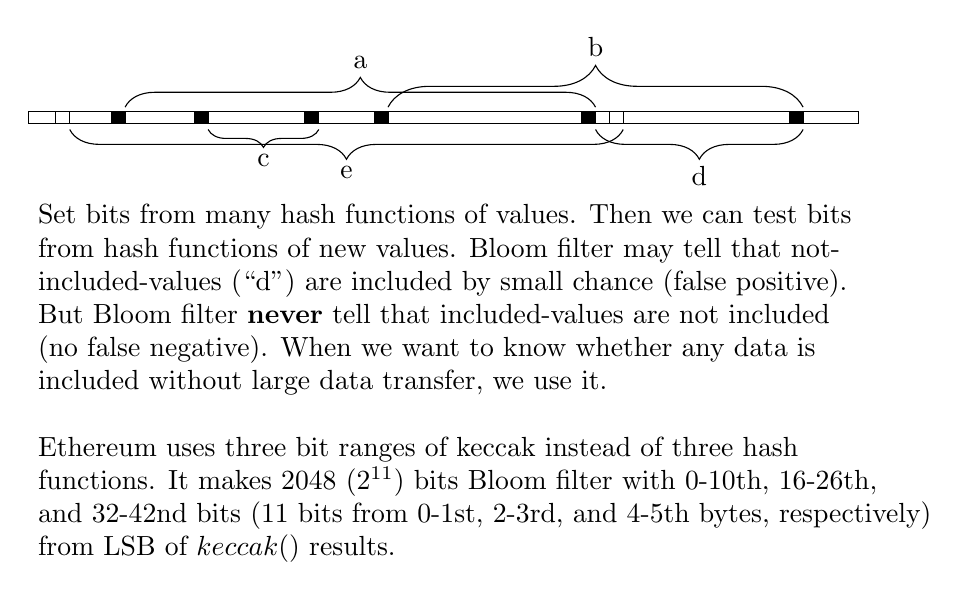
\begin{tikzpicture}[scale=1.0,every node/.style={transform shape}]
    \tikzstyle{field}=[minimum width=6em,minimum height=2.8ex,draw]
    \tikzstyle{desc}=[right=+4em]

\draw (0em,0ex) rectangle (30em,1ex);
\draw (1em,0ex) rectangle (1.5em,1ex) node (e1) {};
\draw[fill] (3em,0ex) rectangle (3.5em,1ex) node (a1) {};
\draw[fill] (6em,0ex) rectangle (6.5em,1ex) node (c1) {};
\draw[fill] (10em,0ex) rectangle (10.5em,1ex) node (c2) {};
\draw[fill] (12.5em,0ex) rectangle (13em,1ex) node (b1) {};
\draw[fill] (20em,0ex) rectangle (20.5em,1ex) node (a2) {};
\draw (21em,0ex) rectangle (21.5em,1ex) node (e2) {};
\draw[fill] (27.5em,0ex) rectangle (28em,1ex) node (b2) {};

% strange behavior of brace decoration
\begin{scope}[/pgf/decoration/raise=-2pt]
\draw[decorate,decoration={brace,amplitude=2.5ex}] (a1.north) -- node[above=2ex] {a} (a2.north);
\draw[decorate,decoration={brace,amplitude=3.5ex}] (b1.north) -- node[above=3ex] {b} (b2.north);
\end{scope}
\begin{scope}[/pgf/decoration/raise=3pt]
\draw[decorate,decoration={brace,amplitude=1.5ex}] (c2.south) -- node[below=2ex] {c} (c1.south);
\draw[decorate,decoration={brace,amplitude=2.5ex}] (b2.south) -- node[below=3ex] {d} (a2.south);
\draw[decorate,decoration={brace,amplitude=2.5ex}] (e2.south) -- node[below=3ex] {e} (e1.south);
\end{scope}

\node[align=left,anchor=north west] at (0em,-6ex) {
Set bits from many hash functions of values. Then we can test bits\\
from hash functions of new values. Bloom filter may tell that not-\\
included-values (``d'') are included by small chance (false positive).\\
But Bloom filter \textbf{never} tell that included-values are not included\\
(no false negative). When we want to know whether any data is\\
included without large data transfer, we use it.\\
\\
Ethereum uses three bit ranges of keccak instead of three hash\\
functions. It makes 2048 (2\textsuperscript{11}) bits Bloom filter with 0-10th, 16-26th,\\
and 32-42nd bits (11 bits from 0-1st, 2-3rd, and 4-5th bytes, respectively)\\
from LSB of $keccak()$ results.
};

  \end{tikzpicture}
\end{frame}